% Options for packages loaded elsewhere
\PassOptionsToPackage{unicode}{hyperref}
\PassOptionsToPackage{hyphens}{url}
%
\documentclass[
]{article}
\usepackage{amsmath,amssymb}
\usepackage{iftex}
\ifPDFTeX
  \usepackage[T1]{fontenc}
  \usepackage[utf8]{inputenc}
  \usepackage{textcomp} % provide euro and other symbols
\else % if luatex or xetex
  \usepackage{unicode-math} % this also loads fontspec
  \defaultfontfeatures{Scale=MatchLowercase}
  \defaultfontfeatures[\rmfamily]{Ligatures=TeX,Scale=1}
\fi
\usepackage{lmodern}
\ifPDFTeX\else
  % xetex/luatex font selection
\fi
% Use upquote if available, for straight quotes in verbatim environments
\IfFileExists{upquote.sty}{\usepackage{upquote}}{}
\IfFileExists{microtype.sty}{% use microtype if available
  \usepackage[]{microtype}
  \UseMicrotypeSet[protrusion]{basicmath} % disable protrusion for tt fonts
}{}
\makeatletter
\@ifundefined{KOMAClassName}{% if non-KOMA class
  \IfFileExists{parskip.sty}{%
    \usepackage{parskip}
  }{% else
    \setlength{\parindent}{0pt}
    \setlength{\parskip}{6pt plus 2pt minus 1pt}}
}{% if KOMA class
  \KOMAoptions{parskip=half}}
\makeatother
\usepackage{xcolor}
\usepackage[margin=1in]{geometry}
\usepackage{color}
\usepackage{fancyvrb}
\newcommand{\VerbBar}{|}
\newcommand{\VERB}{\Verb[commandchars=\\\{\}]}
\DefineVerbatimEnvironment{Highlighting}{Verbatim}{commandchars=\\\{\}}
% Add ',fontsize=\small' for more characters per line
\usepackage{framed}
\definecolor{shadecolor}{RGB}{248,248,248}
\newenvironment{Shaded}{\begin{snugshade}}{\end{snugshade}}
\newcommand{\AlertTok}[1]{\textcolor[rgb]{0.94,0.16,0.16}{#1}}
\newcommand{\AnnotationTok}[1]{\textcolor[rgb]{0.56,0.35,0.01}{\textbf{\textit{#1}}}}
\newcommand{\AttributeTok}[1]{\textcolor[rgb]{0.13,0.29,0.53}{#1}}
\newcommand{\BaseNTok}[1]{\textcolor[rgb]{0.00,0.00,0.81}{#1}}
\newcommand{\BuiltInTok}[1]{#1}
\newcommand{\CharTok}[1]{\textcolor[rgb]{0.31,0.60,0.02}{#1}}
\newcommand{\CommentTok}[1]{\textcolor[rgb]{0.56,0.35,0.01}{\textit{#1}}}
\newcommand{\CommentVarTok}[1]{\textcolor[rgb]{0.56,0.35,0.01}{\textbf{\textit{#1}}}}
\newcommand{\ConstantTok}[1]{\textcolor[rgb]{0.56,0.35,0.01}{#1}}
\newcommand{\ControlFlowTok}[1]{\textcolor[rgb]{0.13,0.29,0.53}{\textbf{#1}}}
\newcommand{\DataTypeTok}[1]{\textcolor[rgb]{0.13,0.29,0.53}{#1}}
\newcommand{\DecValTok}[1]{\textcolor[rgb]{0.00,0.00,0.81}{#1}}
\newcommand{\DocumentationTok}[1]{\textcolor[rgb]{0.56,0.35,0.01}{\textbf{\textit{#1}}}}
\newcommand{\ErrorTok}[1]{\textcolor[rgb]{0.64,0.00,0.00}{\textbf{#1}}}
\newcommand{\ExtensionTok}[1]{#1}
\newcommand{\FloatTok}[1]{\textcolor[rgb]{0.00,0.00,0.81}{#1}}
\newcommand{\FunctionTok}[1]{\textcolor[rgb]{0.13,0.29,0.53}{\textbf{#1}}}
\newcommand{\ImportTok}[1]{#1}
\newcommand{\InformationTok}[1]{\textcolor[rgb]{0.56,0.35,0.01}{\textbf{\textit{#1}}}}
\newcommand{\KeywordTok}[1]{\textcolor[rgb]{0.13,0.29,0.53}{\textbf{#1}}}
\newcommand{\NormalTok}[1]{#1}
\newcommand{\OperatorTok}[1]{\textcolor[rgb]{0.81,0.36,0.00}{\textbf{#1}}}
\newcommand{\OtherTok}[1]{\textcolor[rgb]{0.56,0.35,0.01}{#1}}
\newcommand{\PreprocessorTok}[1]{\textcolor[rgb]{0.56,0.35,0.01}{\textit{#1}}}
\newcommand{\RegionMarkerTok}[1]{#1}
\newcommand{\SpecialCharTok}[1]{\textcolor[rgb]{0.81,0.36,0.00}{\textbf{#1}}}
\newcommand{\SpecialStringTok}[1]{\textcolor[rgb]{0.31,0.60,0.02}{#1}}
\newcommand{\StringTok}[1]{\textcolor[rgb]{0.31,0.60,0.02}{#1}}
\newcommand{\VariableTok}[1]{\textcolor[rgb]{0.00,0.00,0.00}{#1}}
\newcommand{\VerbatimStringTok}[1]{\textcolor[rgb]{0.31,0.60,0.02}{#1}}
\newcommand{\WarningTok}[1]{\textcolor[rgb]{0.56,0.35,0.01}{\textbf{\textit{#1}}}}
\usepackage{graphicx}
\makeatletter
\def\maxwidth{\ifdim\Gin@nat@width>\linewidth\linewidth\else\Gin@nat@width\fi}
\def\maxheight{\ifdim\Gin@nat@height>\textheight\textheight\else\Gin@nat@height\fi}
\makeatother
% Scale images if necessary, so that they will not overflow the page
% margins by default, and it is still possible to overwrite the defaults
% using explicit options in \includegraphics[width, height, ...]{}
\setkeys{Gin}{width=\maxwidth,height=\maxheight,keepaspectratio}
% Set default figure placement to htbp
\makeatletter
\def\fps@figure{htbp}
\makeatother
\setlength{\emergencystretch}{3em} % prevent overfull lines
\providecommand{\tightlist}{%
  \setlength{\itemsep}{0pt}\setlength{\parskip}{0pt}}
\setcounter{secnumdepth}{-\maxdimen} % remove section numbering
\ifLuaTeX
  \usepackage{selnolig}  % disable illegal ligatures
\fi
\IfFileExists{bookmark.sty}{\usepackage{bookmark}}{\usepackage{hyperref}}
\IfFileExists{xurl.sty}{\usepackage{xurl}}{} % add URL line breaks if available
\urlstyle{same}
\hypersetup{
  pdftitle={COMPASS: TEMPEST Discrete DOC Data QAQC},
  pdfauthor={September 2024},
  hidelinks,
  pdfcreator={LaTeX via pandoc}}

\title{COMPASS: TEMPEST Discrete DOC Data QAQC}
\author{September 2024}
\date{2025-06-23}

\begin{document}
\maketitle

\hypertarget{run-information}{%
\subsection{Run Information}\label{run-information}}

\begin{Shaded}
\begin{Highlighting}[]
\CommentTok{\#identify which section you are in }
\FunctionTok{cat}\NormalTok{(}\StringTok{"Run Information"}\NormalTok{)}
\end{Highlighting}
\end{Shaded}

\begin{verbatim}
## Run Information
\end{verbatim}

\begin{Shaded}
\begin{Highlighting}[]
\CommentTok{\#a link to the Gitbook or whatever protocol you are using for this analysis }
  \CommentTok{\#steph will add this soon }
  
\CommentTok{\#anything that needs to be changed do this in the first chunk}
\NormalTok{  Date\_Run }\OtherTok{=} \StringTok{"09/09/24"}
\NormalTok{  Run\_by }\OtherTok{=} \StringTok{"Stephanie J. Wilson"}
\NormalTok{  Script\_run\_by }\OtherTok{=} \StringTok{"Stephanie J. Wilson"}
\NormalTok{  run\_notes }\OtherTok{=} \StringTok{" "}
  
  \CommentTok{\#file path and name for summary file }
\NormalTok{    raw\_file\_name }\OtherTok{=} \StringTok{"tmp\_doc\_raw\_data\_2024/TMP\_202409.txt"} 
  \CommentTok{\#file path and name for the all peaks file }
\NormalTok{    raw\_allpeaks\_name }\OtherTok{=} \StringTok{"tmp\_doc\_raw\_data\_2024/TMP\_202409\_allpeaks.txt"}
  \CommentTok{\#file path and name for processed data after QAQC}
\NormalTok{    processed\_file\_name }\OtherTok{=} \StringTok{"tmp\_doc\_processed\_data\_2024/TMP\_PW\_DOC\_Processed\_202409.csv"}

\CommentTok{\#check standard concentrations {-} Update if running different checks: }
\NormalTok{   chk\_std\_c }\OtherTok{=} \DecValTok{1}
\NormalTok{   chk\_std\_n }\OtherTok{=} \DecValTok{1}
    
\CommentTok{\#Log path }
\NormalTok{    Log\_path }\OtherTok{=} \StringTok{"tmp\_doc\_raw\_data\_2024/COMPASS\_TMP\_TOCTN\_QAQClog\_2024.csv"}
\end{Highlighting}
\end{Shaded}

\hypertarget{setup}{%
\subsection{Setup}\label{setup}}

\hypertarget{pull-in-active-porewater-tracking-inventory-sheet}{%
\subsection{Pull in active porewater tracking inventory
sheet}\label{pull-in-active-porewater-tracking-inventory-sheet}}

\begin{verbatim}
## File already exists. No download needed.
\end{verbatim}

\newpage

\hypertarget{import-data-functions}{%
\subsection{Import Data Functions}\label{import-data-functions}}

\hypertarget{import-sample-data}{%
\subsection{Import Sample Data}\label{import-sample-data}}

\begin{verbatim}
## Import Sample Data
\end{verbatim}

\begin{verbatim}
## New names:
## * `` -> `...14`
\end{verbatim}

\begin{verbatim}
## # A tibble: 3 x 4
##   sample_name    npoc_raw tdn_raw run_datetime        
##   <chr>             <dbl>   <dbl> <chr>               
## 1 TMP_SW_C3_15cm     9.33   0.666 9/10/2024 3:03:33 PM
## 2 TMP_SW_D5_15cm     5.78   0.268 9/10/2024 3:32:19 PM
## 3 TMP_SW_F6_15cm     6.01   0.353 9/10/2024 4:01:16 PM
\end{verbatim}

\newpage

\hypertarget{assessing-standard-curves}{%
\subsection{Assessing standard Curves}\label{assessing-standard-curves}}

\begin{verbatim}
## Assess the Standard Curve
\end{verbatim}

\begin{verbatim}
## New names:
## `geom_smooth()` using formula = 'y ~ x'
## * `` -> `...18`
\end{verbatim}

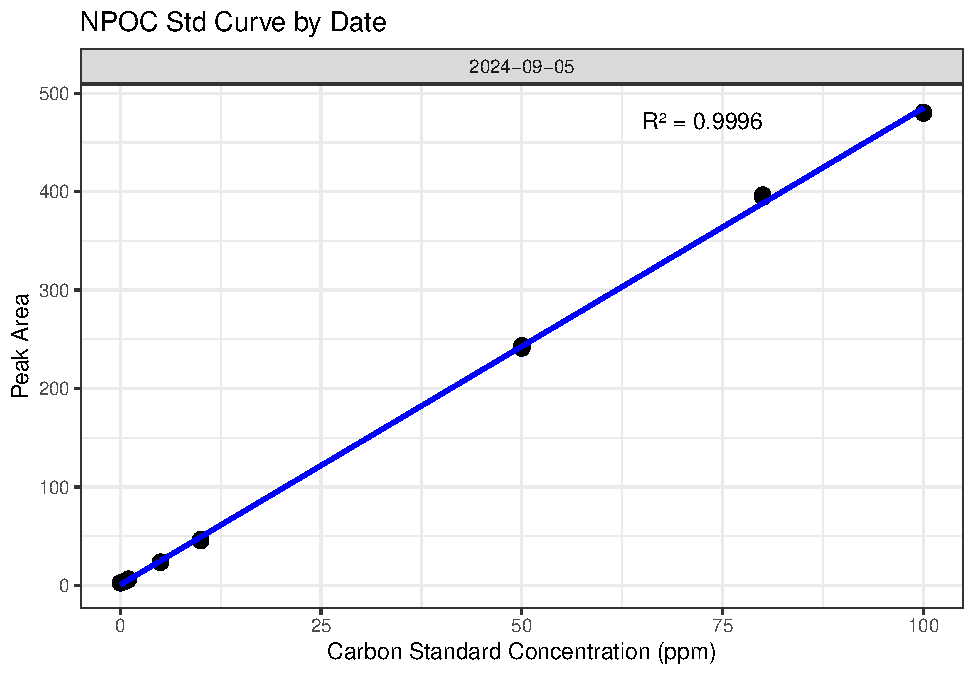
\includegraphics{tmp_doc_discrete_data_processing_202409_files/figure-latex/Assess Standard Curves-1.pdf}

\begin{verbatim}
## `geom_smooth()` using formula = 'y ~ x'
\end{verbatim}

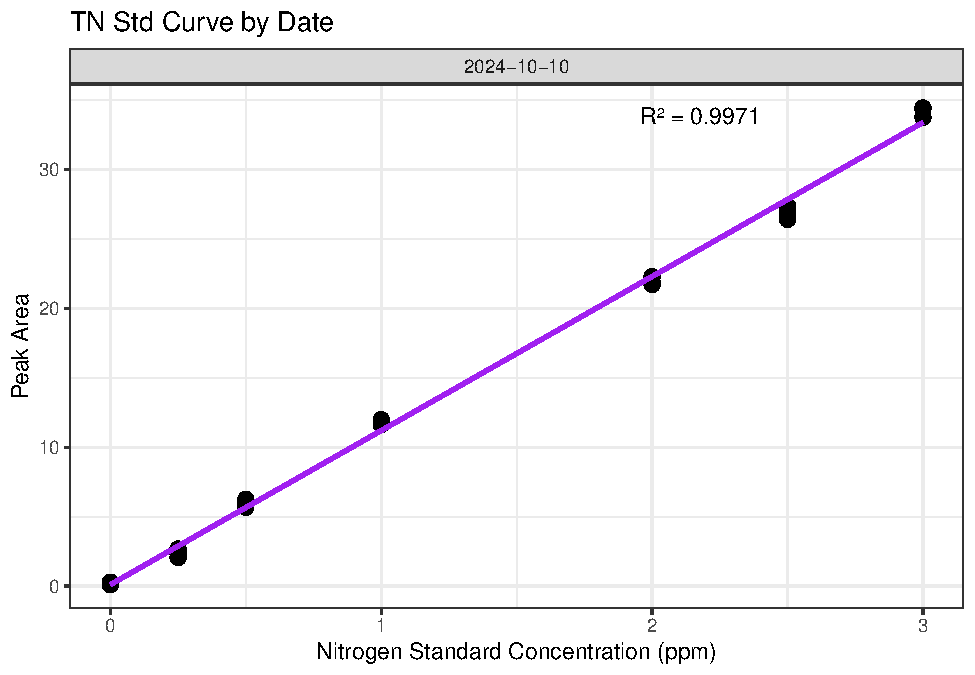
\includegraphics{tmp_doc_discrete_data_processing_202409_files/figure-latex/Assess Standard Curves-2.pdf}

\begin{verbatim}
## Warning: Removed 15 rows containing missing values or values outside the scale range
## (`geom_point()`).
\end{verbatim}

\begin{verbatim}
## Warning: Removed 15 rows containing missing values or values outside the scale range
## (`geom_line()`).
\end{verbatim}

\begin{verbatim}
## `geom_line()`: Each group consists of only one observation.
## i Do you need to adjust the group aesthetic?
\end{verbatim}

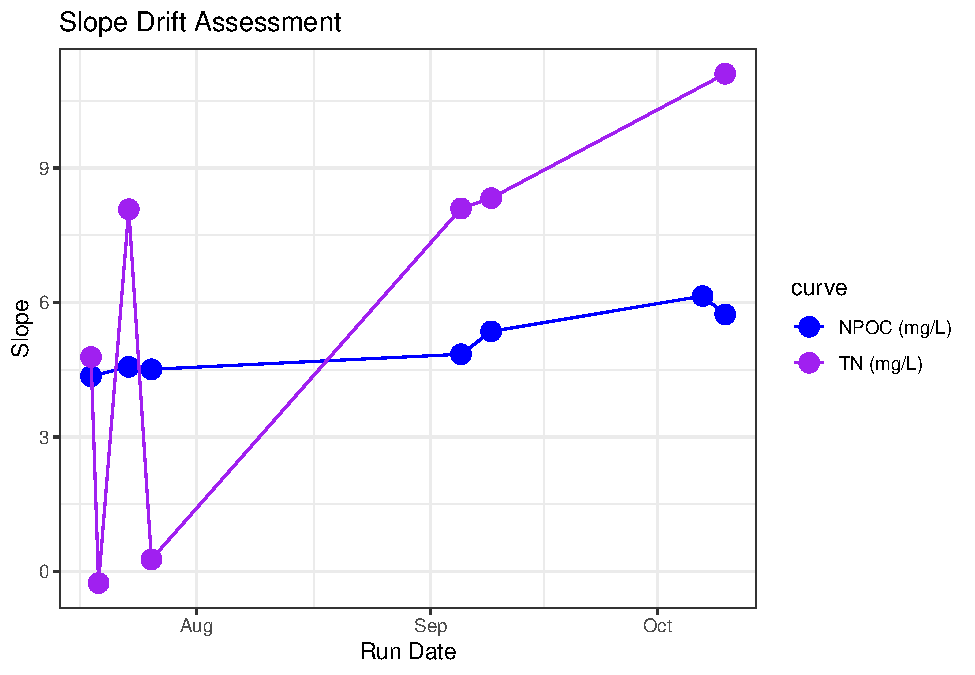
\includegraphics{tmp_doc_discrete_data_processing_202409_files/figure-latex/Assess Standard Curves-3.pdf}

\begin{verbatim}
## [1] "NPOC Curve r2 GOOD"
\end{verbatim}

\begin{verbatim}
## [1] "TN Curve r2 GOOD"
\end{verbatim}

\newpage

\hypertarget{assess-check-standards}{%
\subsection{Assess Check Standards}\label{assess-check-standards}}

\begin{verbatim}
## Assess the Check Standards
\end{verbatim}

\begin{verbatim}
## New names:
## * `` -> `...14`
\end{verbatim}

\begin{verbatim}
## [1] "Carbon CHECK STANDARD RSD TOO HIGH - REASSESS"
\end{verbatim}

\begin{verbatim}
## [1] "Nitrogen CHECK STANDARD RSD TOO HIGH - REASSESS"
\end{verbatim}

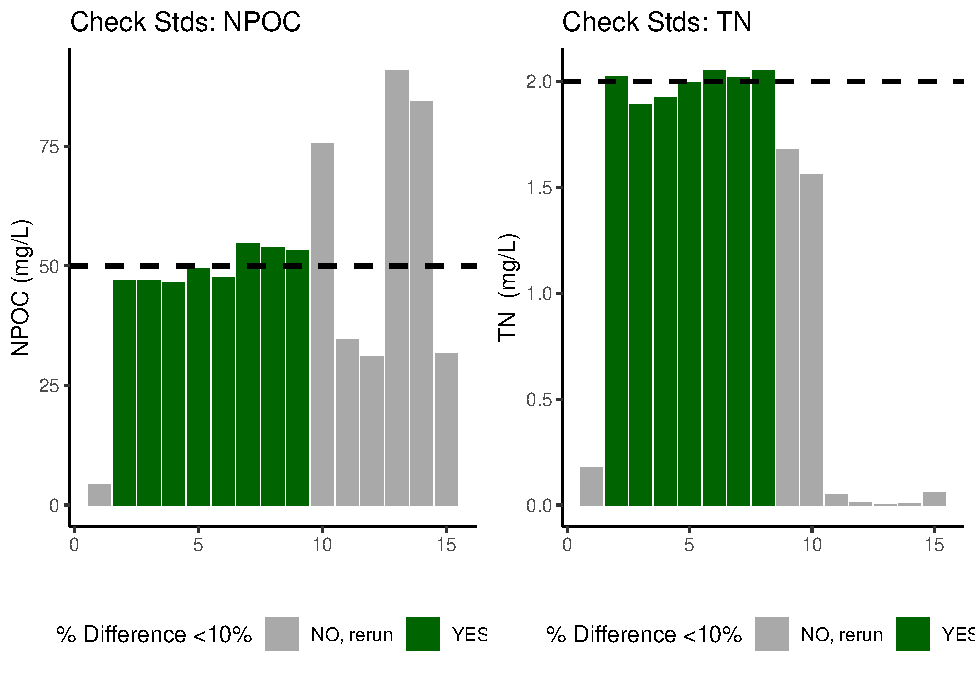
\includegraphics{tmp_doc_discrete_data_processing_202409_files/figure-latex/Check Standards-1.pdf}

\begin{verbatim}
## [1] "<60% of Carbon Check Standards are within range of the expected concentration - REASSESS"
\end{verbatim}

\begin{verbatim}
## [1] "<60% of Nitrogen Check Standards are within range of the expected concentration - REASSESS"
\end{verbatim}

\newpage

\hypertarget{assess-blanks}{%
\subsection{Assess Blanks}\label{assess-blanks}}

\begin{verbatim}
## Assess Blanks
\end{verbatim}

\begin{verbatim}
## New names:
## * `` -> `...14`
\end{verbatim}

\begin{verbatim}
## [1] ">60% of Carbon Blank concentrations are below the lower 25% quartile of samples"
\end{verbatim}

\begin{verbatim}
## [1] ">60% of Nitrogen Blank concentrations are below the lower 25% quartile of samples"
\end{verbatim}

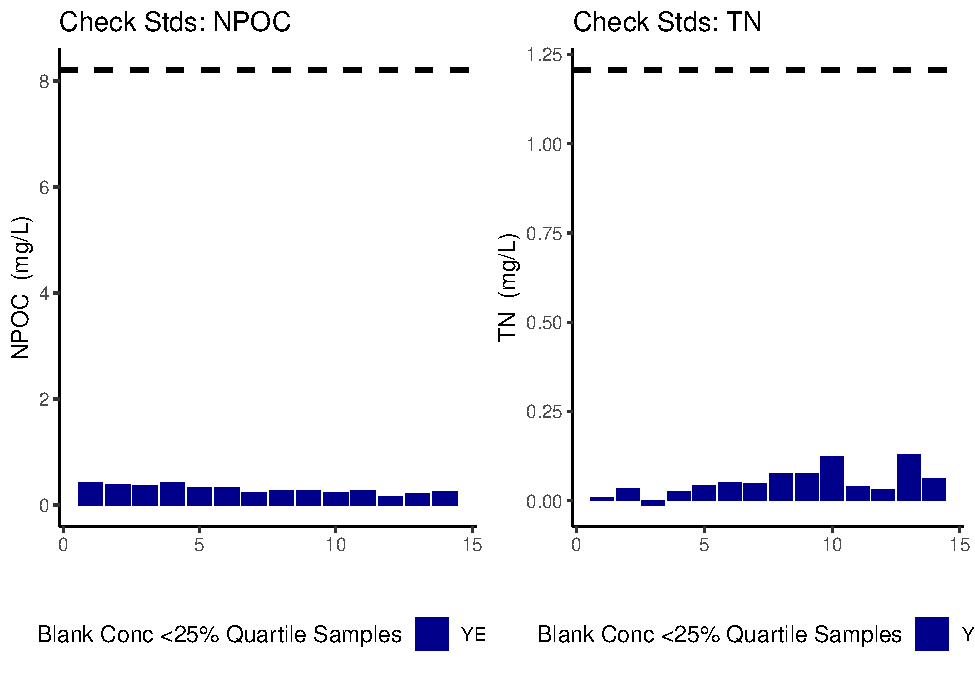
\includegraphics{tmp_doc_discrete_data_processing_202409_files/figure-latex/Check Blanks-1.pdf}

\begin{verbatim}
## carbon blanks:
\end{verbatim}

\begin{verbatim}
## [1] 0.3744933
\end{verbatim}

\begin{verbatim}
## nitrogen blanks:
\end{verbatim}

\begin{verbatim}
## [1] 0.08074067
\end{verbatim}

\newpage

\hypertarget{assess-duplicates---if-there-are-any}{%
\subsection{Assess Duplicates - if there are
any}\label{assess-duplicates---if-there-are-any}}

```\{\#r Check Duplicates, echo=FALSE\}

cat(``Assess Duplicates'')

\#Take a look at the raw data \#head(dat\_raw)

\#pull out any rows that have ``dup'' in the sample\_name column dups
\textless- dat\_raw \%\textgreater\%\\
select(!c(npoc\_flag, tdn\_flag)) \%\textgreater\%
filter(str\_detect(sample\_name, ``dup'')) \#have to change this to
match data

\#create a new dataframe and remove dups from sample dataframe dat\_raw2
\textless- dat\_raw \%\textgreater\%\\
filter(!str\_detect(sample\_name, ``dup''))

\#remove the dup from these IDs so we will have duplicate sample names
dups\(sample_name<-gsub("_dup","",as.character(dups\)sample\_name)) dups
\textless- dups{[} ,-c(4){]} \#remove the run date time for
colnames(dups) \textless- c(`sample\_name', `npoc\_raw\_dup',
``tdn\_raw\_dup'') head(dups)

QAdups \textless- merge(dat\_raw2, dups) head(QAdups)

df2 \textless- as.data.frame(QAdups\(npoc_raw) df2\)dups \textless-
QAdups\$npoc\_raw\_dup

df2\(sds <- apply(df2,1,sd) df2\)mean \textless- apply(df2, 1, mean)

QAdups\(npoc_dups_cv <- (df2\)sds/df2\(mean) * 100 QAdups\)npoc\_dups\_cv\_flag
\textless- ifelse(QAdups\$npoc\_dups\_cv \textless10, `YES', `NO,
rerun')

df3 \textless- as.data.frame(QAdups\(tdn_raw) df3\)dups \textless-
QAdups\$tdn\_raw\_dup

df3\(sds <- apply(df3,1,sd) df3\)mean \textless- apply(df3, 1, mean)

QAdups\(tdn_dups_cv <- (df3\)sds/df3\(mean) * 100 QAdups\)tdn\_dups\_cv\_flag
\textless- ifelse(QAdups\$tdn\_dups\_cv \textless10, `YES', `NO, rerun')

head(QAdups)

\#plot dups output as a bar graph to easily check - want any over 10\%
to be red need to work on this C\_dups \textless- ggplot(data =QAdups,
aes(x =sample\_name, y =npoc\_dups\_cv, fill=npoc\_dups\_cv\_flag)) +
geom\_bar(stat = `identity') + theme\_classic() + labs(x= ``Sample ID'',
y=``CV of NPOC Dups (\%)'') + scale\_fill\_manual(values = c(``YES'' =
``darkgreen'', ``NO, rerun'' = ``red'')) +
theme(legend.position=``none'') + geom\_hline(yintercept=10,
linetype=``dashed'', color = ``black'', size=1) +
guides(fill=guide\_legend(title=``CV Between Dups \textless10\%'')) +
theme(axis.text.x = element\_text(angle = 90, hjust = 0.5))

N\_dups \textless- ggplot(data =QAdups, aes(x =sample\_name, y
=tdn\_dups\_cv, fill=tdn\_dups\_cv\_flag)) + geom\_bar(stat =
`identity') + theme\_classic() + labs(x= ``Sample ID'', y=``CV of TN
Dups (\%)'') + scale\_fill\_manual(values = c(``YES'' = ``darkgreen'',
``NO, rerun'' = ``red'')) + theme(legend.position=``none'') +
geom\_hline(yintercept=10, linetype=``dashed'', color = ``black'',
size=1) + guides(fill=guide\_legend(title=``CV Between Dups
\textless10\%''))+ theme(axis.text.x = element\_text(angle = 90, hjust =
0.5))

ggarrange(C\_dups, N\_dups,ncol=2, nrow=1)

\#calculate the percent of check standards that are within the range
based on the flag c\_dups\_percent \textless-
(sum(QAdups\(npoc_dups_cv_flag == "YES")/nrow(QAdups))*100 n_dups_percent <- (sum(QAdups\)tdn\_dups\_cv\_flag
== ``YES'')/nrow(QAdups))*100

\#report out if flags indicate need for rerun ifelse(c\_dups\_percent
\textgreater= chks\_flag, ``\textgreater60\% of Carbon Duplicates have a
CV \textless10\%'', ``\textless60\% of Carbon Duplicates have a CB
\textless10\% - REASSESS'') ifelse(n\_dups\_percent \textgreater=
chks\_flag, ``\textgreater60\% of Nitrogen Duplicates have a CV
\textless10\%'', ``\textless60\% of Nitrogen Duplicates have a CB
\textless10\% - REASSESS'')

\#write out a flag to the sample dataframe if more than 60\% of the dups
have CVs out of range if (c\_dups\_percent \textless= chks\_flag) \{
dat\_raw\(npoc_flag <- ifelse(  dat_raw\)npoc\_flag != ````,
paste0(dat\_raw\$npoc\_flag,''; NPOC dups out of range''), ``NPOC dups
out of range'' ) \}

if (n\_dups\_percent \textless= chks\_flag) \{ \# assuming you have
tn\_chks\_percent similarly
dat\_raw\(tdn_flag <- ifelse(  dat_raw\)tdn\_flag != ````,
paste0(dat\_raw\$tdn\_flag,''; TN dups out of range''), ``TN dups out of
range'' ) \}

\begin{verbatim}

\newpage

## Sample Flagging   
\end{verbatim}

\hypertarget{sample-flagging}{%
\subsection{Sample Flagging}\label{sample-flagging}}

\begin{verbatim}

![](tmp_doc_discrete_data_processing_202409_files/figure-latex/Sample Flagging-1.pdf)<!-- --> ![](tmp_doc_discrete_data_processing_202409_files/figure-latex/Sample Flagging-2.pdf)<!-- --> 

\newpage

## Visualize Data by Plot   
\end{verbatim}

\hypertarget{visualize-data}{%
\subsection{Visualize Data}\label{visualize-data}}

\begin{verbatim}
\end{verbatim}

\hypertarget{site_code-plot-grid_square-date}{%
\subsection{Site\_Code Plot Grid\_Square
Date}\label{site_code-plot-grid_square-date}}

\hypertarget{tmp-sw-c3-15cm}{%
\subsection{1 TMP SW C3 15cm}\label{tmp-sw-c3-15cm}}

\hypertarget{tmp-sw-d5-15cm}{%
\subsection{2 TMP SW D5 15cm}\label{tmp-sw-d5-15cm}}

\hypertarget{tmp-sw-f6-15cm}{%
\subsection{3 TMP SW F6 15cm}\label{tmp-sw-f6-15cm}}

\begin{verbatim}
\end{verbatim}

\hypertarget{site_code-plot-grid_square-date-sample_name-npoc_raw-tdn_raw}{%
\subsection{Site\_Code Plot Grid\_Square Date sample\_name npoc\_raw
tdn\_raw}\label{site_code-plot-grid_square-date-sample_name-npoc_raw-tdn_raw}}

\hypertarget{tmp-sw-c3-15cm-tmp_sw_c3_15cm-9.329-0.6664}{%
\subsection{1 TMP SW C3 15cm TMP\_SW\_C3\_15cm 9.329
0.6664}\label{tmp-sw-c3-15cm-tmp_sw_c3_15cm-9.329-0.6664}}

\hypertarget{tmp-sw-d5-15cm-tmp_sw_d5_15cm-5.781-0.2683}{%
\subsection{2 TMP SW D5 15cm TMP\_SW\_D5\_15cm 5.781
0.2683}\label{tmp-sw-d5-15cm-tmp_sw_d5_15cm-5.781-0.2683}}

\hypertarget{tmp-sw-f6-15cm-tmp_sw_f6_15cm-6.013-0.3530}{%
\subsection{3 TMP SW F6 15cm TMP\_SW\_F6\_15cm 6.013
0.3530}\label{tmp-sw-f6-15cm-tmp_sw_f6_15cm-6.013-0.3530}}

\hypertarget{run_datetime-npoc_flag}{%
\subsection{run\_datetime npoc\_flag}\label{run_datetime-npoc_flag}}

\hypertarget{pm-npoc-checks-out-of-range}{%
\subsection{1 9/10/2024 3:03:33 PM NPOC checks out of
range}\label{pm-npoc-checks-out-of-range}}

\hypertarget{pm-npoc-checks-out-of-range-1}{%
\subsection{2 9/10/2024 3:32:19 PM NPOC checks out of
range}\label{pm-npoc-checks-out-of-range-1}}

\hypertarget{pm-npoc-checks-out-of-range-2}{%
\subsection{3 9/10/2024 4:01:16 PM NPOC checks out of
range}\label{pm-npoc-checks-out-of-range-2}}

\hypertarget{tdn_flag}{%
\subsection{tdn\_flag}\label{tdn_flag}}

\hypertarget{tn-checks-out-of-range}{%
\subsection{1 TN checks out of range}\label{tn-checks-out-of-range}}

\hypertarget{tn-checks-out-of-range-blank-is-25-of-sample-value}{%
\subsection{2 TN checks out of range; blank is ≥ 25\% of sample
value}\label{tn-checks-out-of-range-blank-is-25-of-sample-value}}

\hypertarget{tn-checks-out-of-range-1}{%
\subsection{3 TN checks out of range}\label{tn-checks-out-of-range-1}}

\begin{verbatim}

![](tmp_doc_discrete_data_processing_202409_files/figure-latex/Visualize Data-1.pdf)<!-- --> ![](tmp_doc_discrete_data_processing_202409_files/figure-latex/Visualize Data-2.pdf)<!-- --> 

\newpage

## Convert data from mg/L to uMoles/L 


## Add in/check metadata 
\end{verbatim}

\hypertarget{check-sample-ids-with-metadata}{%
\subsection{Check Sample IDs with
Metadata}\label{check-sample-ids-with-metadata}}

\begin{verbatim}
\end{verbatim}

\hypertarget{a-tibble-3-x-2}{%
\subsection{\# A tibble: 3 x 2}\label{a-tibble-3-x-2}}

\hypertarget{sample_name-metadata_recorded}{%
\subsection{sample\_name
metadata\_recorded}\label{sample_name-metadata_recorded}}

\hypertarget{section}{%
\subsection{\texorpdfstring{ }{ }}\label{section}}

\hypertarget{tmp_sw_c3_15cm-false}{%
\subsection{1 TMP\_SW\_C3\_15cm FALSE}\label{tmp_sw_c3_15cm-false}}

\hypertarget{tmp_sw_d5_15cm-false}{%
\subsection{2 TMP\_SW\_D5\_15cm FALSE}\label{tmp_sw_d5_15cm-false}}

\hypertarget{tmp_sw_f6_15cm-false}{%
\subsection{3 TMP\_SW\_F6\_15cm FALSE}\label{tmp_sw_f6_15cm-false}}

\begin{verbatim}

## Export Processed Data  
\end{verbatim}

\hypertarget{export-processed-data}{%
\subsection{Export Processed Data}\label{export-processed-data}}

\begin{verbatim}
\end{verbatim}

\hypertarget{a-tibble-3-x-21}{%
\subsection{\# A tibble: 3 x 21}\label{a-tibble-3-x-21}}

\hypertarget{project-plot-grid-depth_cm-sample_type-vial_id-date-npoc_mgl-npoc_um}{%
\subsection{Project plot grid Depth\_cm sample\_type Vial\_ID date
npoc\_mgL
npoc\_uM}\label{project-plot-grid-depth_cm-sample_type-vial_id-date-npoc_mgl-npoc_um}}

\hypertarget{section-1}{%
\subsection{\texorpdfstring{ }{        }}\label{section-1}}

\hypertarget{section-2}{%
\subsection{\texorpdfstring{1 15 9.33
777.}{1    15    9.33 777.}}\label{section-2}}

\hypertarget{section-3}{%
\subsection{\texorpdfstring{2 15 5.78
482.}{2    15    5.78 482.}}\label{section-3}}

\hypertarget{section-4}{%
\subsection{\texorpdfstring{3 15 6.01
501.}{3    15    6.01 501.}}\label{section-4}}

\hypertarget{i-12-more-variables-npoc_flag-tdn_mgl-tdn_um}{%
\subsection{\# i 12 more variables: npoc\_flag , tdn\_mgL , tdn\_uM
,}\label{i-12-more-variables-npoc_flag-tdn_mgl-tdn_um}}

\hypertarget{tdn_flag-analysis_runtime-run_notes}{%
\subsection{\# tdn\_flag , Analysis\_runtime , Run\_notes
,}\label{tdn_flag-analysis_runtime-run_notes}}

\hypertarget{evacuation_date_yyymmdd-collection_date_yyyymmdd}{%
\subsection{\# Evacuation\_date\_YYYMMDD , Collection\_Date\_YYYYMMDD
,}\label{evacuation_date_yyymmdd-collection_date_yyyymmdd}}

\hypertarget{collection_start_time_24hrs-collection_end_time_24hrs}{%
\subsection{\# Collection\_Start\_Time\_24hrs ,
Collection\_End\_Time\_24hrs
,}\label{collection_start_time_24hrs-collection_end_time_24hrs}}

\hypertarget{est_edt-volume_ml}{%
\subsection{\texorpdfstring{\# EST\_EDT , Volume\_mL
}{\# EST\_EDT , Volume\_mL }}\label{est_edt-volume_ml}}

```

\#end

\end{document}
